%%%%%%%%%%%%%%%%%%%%%%%%%%%%%%%%%%%%%%%%%
% Short Sectioned Assignment
% LaTeX Template
% Version 1.0 (5/5/12)
%
% This template has been downloaded from:
% http://www.LaTeXTemplates.com
%
% Original author:
% Frits Wenneker (http://www.howtotex.com)
%
% License:
% CC BY-NC-SA 3.0 (http://creativecommons.org/licenses/by-nc-sa/3.0/)
%
%%%%%%%%%%%%%%%%%%%%%%%%%%%%%%%%%%%%%%%%%

%----------------------------------------------------------------------------------------
%	PACKAGES AND OTHER DOCUMENT CONFIGURATIONS
%----------------------------------------------------------------------------------------

\documentclass[paper=a4, fontsize=11pt]{scrartcl} % A4 paper and 11pt font size

\usepackage[T1]{fontenc} % Use 8-bit encoding that has 256 glyphs
\usepackage{fourier} % Use the Adobe Utopia font for the document - comment this line to return to the LaTeX default
\usepackage[english]{babel} % English language/hyphenation
\usepackage{amsmath,amsfonts,amsthm} % Math packages

\usepackage{graphicx}

\usepackage{sectsty} % Allows customizing section commands
\allsectionsfont{\centering \normalfont\scshape} % Make all sections centered, the default font and small caps

\usepackage{fancyhdr} % Custom headers and footers
\pagestyle{fancyplain} % Makes all pages in the document conform to the custom headers and footers
\fancyhead{} % No page header - if you want one, create it in the same way as the footers below
\fancyfoot[L]{} % Empty left footer
\fancyfoot[C]{} % Empty center footer
\fancyfoot[R]{\thepage} % Page numbering for right footer
\renewcommand{\headrulewidth}{0pt} % Remove header underlines
\renewcommand{\footrulewidth}{0pt} % Remove footer underlines
\setlength{\headheight}{13.6pt} % Customize the height of the header

\numberwithin{equation}{section} % Number equations within sections (i.e. 1.1, 1.2, 2.1, 2.2 instead of 1, 2, 3, 4)
\numberwithin{figure}{section} % Number figures within sections (i.e. 1.1, 1.2, 2.1, 2.2 instead of 1, 2, 3, 4)
\numberwithin{table}{section} % Number tables within sections (i.e. 1.1, 1.2, 2.1, 2.2 instead of 1, 2, 3, 4)

\setlength\parindent{0pt} % Removes all indentation from paragraphs - comment this line for an assignment with lots of text

%----------------------------------------------------------------------------------------
%	TITLE SECTION
%----------------------------------------------------------------------------------------

\newcommand{\horrule}[1]{\rule{\linewidth}{#1}} % Create horizontal rule command with 1 argument of height

\title{	
\normalfont \normalsize 
\textsc{Bonn-Rhein-Sieg University of Applied Sciences} \\ [25pt] % Your university, school and/or department name(s)
\horrule{0.5pt} \\[0.4cm] % Thin top horizontal rule
\huge Scientific Experimentation and Evaluation\\
- Assignment 01 - \\ % The assignment title
\horrule{2pt} \\[0.5cm] % Thick bottom horizontal rule
}

\author{Bastian Lang, Mazin Eltayeb} % Your name

\date{\normalsize\today} % Today's date or a custom date

\begin{document}

\maketitle % Print the title

\tableofcontents
\newpage

\section{Design of Experiment}
\subsection{Consider how to best record the end poses of the three times 20 runs of the robot.}
This experiment is about getting a model of the movement of robot. 
So we are interested in the end pose of the robot after applying a motion command to a robot standing in the start pose. 
As for one part's position of the robot will not be enough to specify the orientation of the robot, we consider the positions of all three wheels when specifying the pose of a robot.

To measure the end position of the robot, we need to specify and record the end pose of the robot with respect to some coordinate system. 
As for we are interested in the movement with respect to the starting pose, we define this as the origin of our system.

To reduce measurement errors and make the measurement process easier, we use a grid on the paper ground. 
To avoid to much (unnecessary) work in advance we use a coarse grid of 10cm x 10cm sized cells. 
To determine the exact position we use a ruler within these cells.

\subsubsection{Experimental Terms}

	\textbf{Measurement System}
	\begin{itemize}
		\item The ground paper with the grid
		\item Measurement tools (ruler)
		\item Robot
	\end{itemize}
	\textbf{Measuring Facility}
	\begin{itemize}
		\item The ground paper with the grid (see figure \ref{facility})
		\item Measurement tools (ruler)
	\end{itemize}
	\textbf{Measurand:}
	\begin{itemize}
		\item Travelled distance
	\end{itemize}
	\textbf{Measured (quantity) values:}
	\begin{itemize}
		\item Position of left wheel
		\item Position of right wheel
		\item Position of front wheel
	\end{itemize}
	\textbf{Measurement Result:}
	\begin{itemize}
		\item Robots end pose specified by three wheel-positions
	\end{itemize}
	\textbf{Device under Test (DUT):}
	\begin{itemize}
		\item Robot (see figure \ref{fig_5_min_bot})
	\end{itemize}
	\textbf{Sensitivity:}
	\begin{itemize}
		\item Millimeters
	\end{itemize}
	\textbf{Display:}
	\begin{itemize}
		\item Gridded paper ground
	\end{itemize}



\subsection{Describe in writing the robots design, the measurement process and the expected problems.}
\begin{figure}[ht]
	\centering
  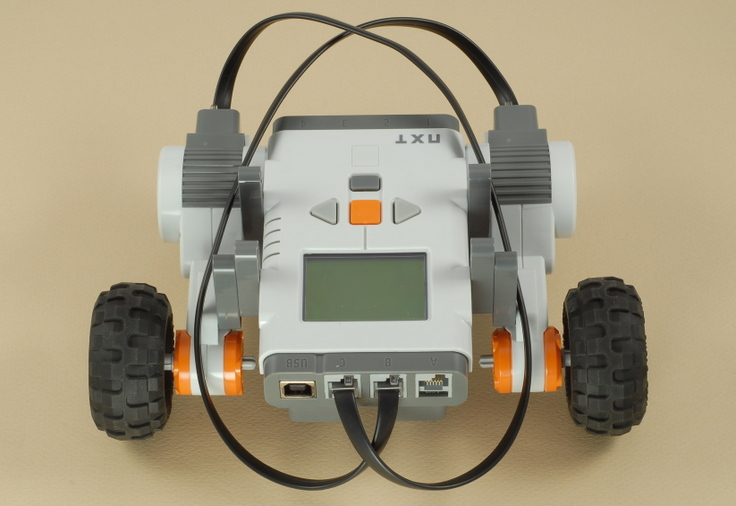
\includegraphics[width=0.5\textwidth]{5min_bot.JPG}
	\caption{The five minutes robot : http://www.nxtprograms.com/five\textunderscore minute\textunderscore bot/DCP\textunderscore 8899.JPG}
	\label{fig_5_min_bot}
\end{figure}

\begin{figure}[ht]
	\centering
  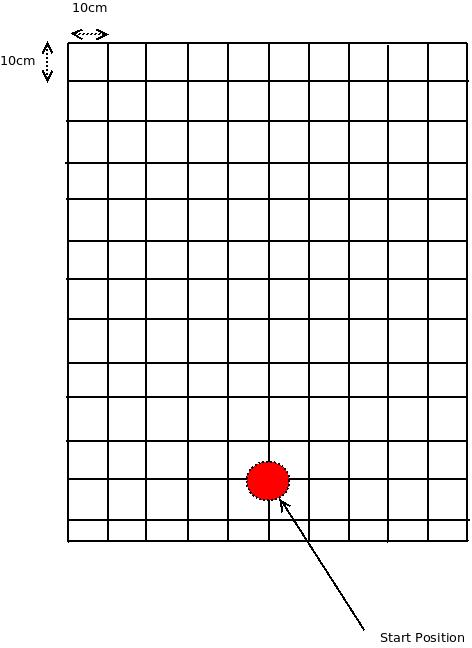
\includegraphics[width=0.5\textwidth]{facility.jpeg}
	\caption{The measurement facility: gridded paper}
	\label{fig_facility}
\end{figure}
\subsubsection{The Robot's Design}
Our robot is the 5 minutes bot as can be seen in figure \ref{fig_5_min_bot}.
It consists of two actuated wheels on the sides of the robot and one free spinning wheel in the front.

\subsubsection{The Measurement Process}
We first fix and mark the robot's starting pose on the paper ground.
For each run we place the robot's wheels exactly on their marks and run the movement program.
After the robot has reached its end position, we mark the wheel positions and then use our grid and a ruler to get the values of their positions.
Each value gets recorded.

\subsubsection{Expected Problems}
One problem will be the exact measurement of the wheel poses. 
There will probably already be small inaccuracies when marking the wheel positions, but also using the ruler to determine the values of the positions will yield additional inaccuracies.

Another problem will be the exact positioning of the robot in the start pose.

\subsection{Give a rough (but justified by some arguments) estimation of the expected accuracy and precision of your measurement process.}
As humans we are probably able to place the robot in its start pose and to mark its end pose with only a few (~5mm) millimeters off. The measurement using a ruler and our grid will probably hold another one or two millimeters. 
So we expect errors within the range of roughly a centimeter.






\end{document}